% This LaTeX document needs to be compiled with XeLaTeX.
\documentclass[10pt]{article}
\usepackage[utf8]{inputenc}
\usepackage{graphicx}
\usepackage[export]{adjustbox}
\graphicspath{ {./images/} }
\usepackage{amsmath}
\usepackage{amsfonts}
\usepackage{amssymb}
\usepackage[version=4]{mhchem}
\usepackage{stmaryrd}
\usepackage{multirow}
\usepackage[fallback]{xeCJK}
\usepackage{polyglossia}
\usepackage{fontspec}
\setCJKmainfont{Noto Serif CJK JP}

\setmainlanguage{polish}
\setmainfont{CMU Serif}

\title{KOD }

\author{}
\date{}


\begin{document}
\maketitle
\section*{PESEL}
\begin{center}

\includegraphics[max width=\textwidth]{2024_11_21_9a9f600c3b3af5013d80g-01(2)}
\end{center}

PRÓBNY EGZAMIN MATURALNY

\section*{Z MATEMATYKI}
\section*{POZIOM PODSTAWOWY}
\begin{enumerate}
  \item Sprawdź, czy arkusz egzaminacyjny zawiera 16 stron (zadania 1-34). Ewentualny brak zgłoś przewodniczącemu zespołu nadzorującego próbny egzamin.
  \item Rozwiązania zadań i odpowiedzi wpisuj w miejscu na to przeznaczonym.
  \item Odpowiedzi do zadań zamkniętych (1-25) przenieś na kartę odpowiedzi, zaznaczając je w części karty przeznaczonej dla zdającego. Zamaluj - pola do tego przeznaczone. Błędne zaznaczenie otocz kółkiem i zaznacz właściwe.
  \item Pamiętaj, że pominięcie argumentacji lub istotnych obliczeń w rozwiązaniu zadania otwartego (26-34) może spowodować, że za to rozwiązanie nie będziesz mógł dostać pełnej liczby punktów.
  \item Pisz czytelnie i używaj tylko długopisu lub pióra z czarnym tuszem lub atramentem.
  \item Nie używaj korektora, a błędne zapisy wyraźnie przekreśl.
  \item Pamiętaj, że zapisy w brudnopisie nie będą oceniane.
  \item Możesz korzystać z zestawu wzorów matematycznych, cyrkla i linijki oraz kalkulatora.
  \item Na karcie odpowiedzi wpisz swój numer PESEL.
  \item Nie wpisuj żadnych znaków w części przeznaczonej dla egzaminatora.
\end{enumerate}

We wspólpracy\\

\includegraphics[max width=\textwidth, center]{2024_11_21_9a9f600c3b3af5013d80g-01}\\
centrum\\

\includegraphics[max width=\textwidth, center]{2024_11_21_9a9f600c3b3af5013d80g-01(1)}

Luty 2013

Czas pracy:\\
170 minut

Liczba punktów\\
do uzyskania: 50

\section*{ZADANIA ZAMKNIĘTE}
\section*{W zadaniach od 1. do 25. wybierz i zaznacz na karcie odpowiedzi poprawna odpowiedź}
Zadanie 1. (1 pkt)\\
Wskaż liczbę, której 0,4\% jest równe 12.\\
A. 0,048\\
B. 0,48\\
C. 30\\
D. 3000

Zadanie 2. (1 pkt)\\
Dane są wielomiany \(w(x)=-3 \mathrm{x}^{3}-5 \mathrm{x}^{2}+\mathrm{x}\) oraz \(v(x)=\mathrm{x}^{3}+2 \mathrm{x}^{2}-6 \mathrm{x}+1\). Wówczas wielomian \(p(x)=-2 w(x)-v(x)\) jest równy:\\
A. \(p(x)=5 \mathrm{x}^{3}+12 \mathrm{x}^{2}-8 \mathrm{x}+1\)\\
B. \(p(x)=-5 x^{3}-12 x^{2}+8 x-1\)\\
C. \(p(x)=5 x^{3}+8 x^{2}+4 x-1\)\\
D. \(p(x)=-7 x^{3}-8 x^{2}-4 x+1\)

Zadanie 3. (1 pkt)\\
Zbiorem wartości funkcji, której wykres przedstawiono na rysunku jest przedział:\\
A. \(\langle-4,5\rangle\)\\
B. \(\langle-3,4\rangle\)\\
C. \(\langle-2,4\rangle\)\\
D. \(\langle-3,2\rangle\)

Zadanie 4. (1 pkt)\\
Który wyraz ciągu \(a_{n}=-\frac{7}{3} n+21\) jest równy zero?\\
A. \(a_{9}\)\\
B. \(a_{18}\)\\
C. \(a_{21}\)\\
D. \(a_{49}\)

Zadanie 5. (1 pkt)\\
Przyprostokątne trójkąta prostokątnego mają długości 3 i 9. Sinus najmniejszego kąta tego trójkąta jest równy:\\
A. \(\frac{3 \sqrt{10}}{10}\)\\
B. \(\frac{1}{3}\)\\
C. \(\frac{\sqrt{10}}{10}\)\\
D. \(\frac{\sqrt{10}}{30}\)

Zadanie 6. (1 pkt)\\
Wzorem funkcji kwadratowej \(f\), której fragment wykresu przedstawiono na rysunku jest:\\
A. \(f(x)=-\frac{1}{2} x^{2}+2 x-1\)\\
B. \(f(x)=-\frac{1}{2} x^{2}+2 x+1\)\\
C. \(f(x)=-\frac{1}{2} x^{2}+x+1\)\\
D. \(f(x)=-\frac{1}{2} x^{2}-2 x+1\)

Zadanie 7. (1 pkt)\\
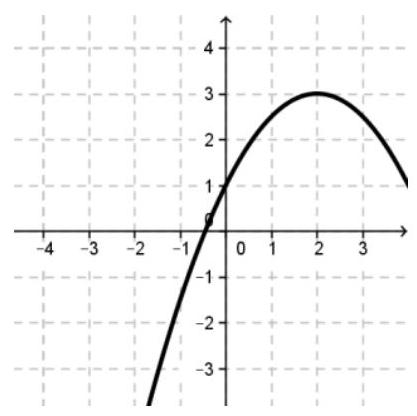
\includegraphics[max width=\textwidth, center]{2024_11_21_9a9f600c3b3af5013d80g-02}

Wyrażenie \(\sqrt[3]{9} \cdot \sqrt[5]{27}\) zapisane w postaci potęgi liczby 3 jest równe:\\
A. \(3^{\frac{2}{5}}\)\\
B. \(3^{\frac{5}{8}}\)\\
C. \(3^{\frac{19}{15}}\)\\
D. \(3^{\frac{8}{5}}\)

\section*{BRUDNOPIS}
\(\qquad\)

Zadanie 8. (1 pkt)\\
Interpretację geometryczną układu równań \(\left\{\begin{array}{c}x-y=2 \\ -2 x+2 y=4\end{array}\right.\) przedstawiono na rysunku:\\
A.\\
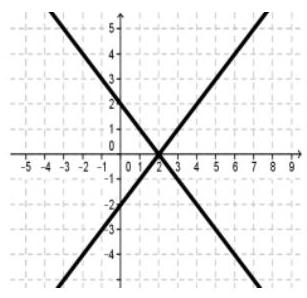
\includegraphics[max width=\textwidth, center]{2024_11_21_9a9f600c3b3af5013d80g-04(3)}\\
B.\\
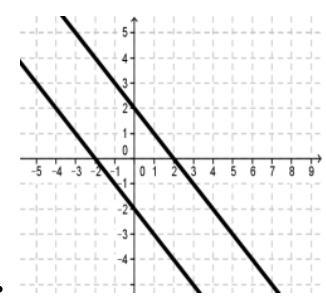
\includegraphics[max width=\textwidth, center]{2024_11_21_9a9f600c3b3af5013d80g-04(1)}\\
C.\\
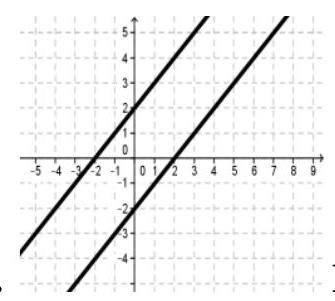
\includegraphics[max width=\textwidth, center]{2024_11_21_9a9f600c3b3af5013d80g-04(4)}\\
D.\\
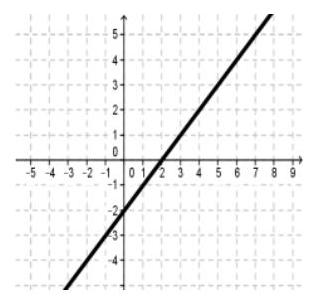
\includegraphics[max width=\textwidth, center]{2024_11_21_9a9f600c3b3af5013d80g-04}

Zadanie 9. (1 pkt)\\
Wielomian \(w(x)=x^{3}-5 x^{2}-3 x+15\) rozłożony na czynniki ma postać\\
A. \(w(x)=(x-3)(x+3)(x-5)\)\\
B. \(w(x)=(x-5)(x+5)\left(x^{2}-3\right)\)\\
C. \(w(x)=(x-5)(x-5)\left(x^{2}-3\right)\)\\
D. \(w(x)=(x-\sqrt{3})(x+\sqrt{3})(x-5)\)

Zadanie 10. (1 pkt)\\
W loterii liczbowej wylosowano dziesięć liczb: 4, 3, 3,3,4,6,1,5,1,6. Mediana tych danych jest równa:\\
A. 5\\
B. 3,6\\
C. 3,5\\
D. 3

Zadanie 11. (1 pkt)\\
Punkt \(S\) jest środkiem koła. Zatem miara kąta \(\alpha\) jest równa (patrz na rysunek obok):\\
A. \(70^{\circ}\)\\
B. \(220^{\circ}\)\\
C. \(140^{\circ}\)\\
D. \(250^{\circ}\)\\
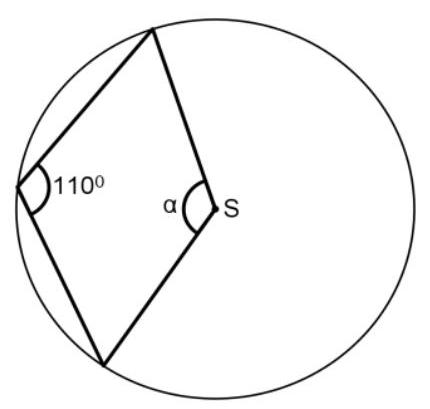
\includegraphics[max width=\textwidth, center]{2024_11_21_9a9f600c3b3af5013d80g-04(2)}

Zadanie 12. (1 pkt)\\
Prostymi równoległymi są wykresy funkcji liniowych:\\
A. \(y=\frac{4}{3} x+5\) i \(y=-\frac{3}{4} x+5\)\\
B. \(y=\frac{4}{3} x+5\) i \(y=-\frac{4}{3} x+5\)\\
C. \(y=\frac{4}{3} x+5\) i \(y=\frac{3}{4} x-5\)\\
D. \(y=\frac{4}{3} x+5\) i \(y=\frac{4}{3} x-5\)

Zadanie 13. (1 pkt)\\
Liczba \(-\frac{3}{2} \log 4+\frac{5}{3} \log 8\) jest równa:\\
A. \(2 \log 2\)\\
B. \(\log 24\)\\
C. 2\\
D. \(8 \log 2\)

Zadanie 14. (1 pkt)\\
Dziedziną funkcji \(f(x)=\frac{x^{2}-16}{(x-2)(x+4)}\) jest zbiór:\\
A. \(R \backslash\{-2,4\}\)\\
B. \(R \backslash\{2,-4\}\)\\
C. \(R \backslash\{-4,4\}\)\\
D. \(R \backslash\{2\}\)

\begin{center}
\begin{tabular}{|c|c|c|c|c|c|c|c|c|c|c|c|c|c|c|c|c|c|c|c|c|c|c|c|}
\hline
 &  &  &  &  &  &  &  &  &  &  &  &  &  &  &  &  &  &  &  &  &  &  &  \\
\hline
 &  &  &  &  &  &  &  &  &  &  &  &  &  &  &  &  &  &  &  &  &  &  &  \\
\hline
 &  &  &  &  &  &  &  &  &  &  &  &  &  &  &  &  &  &  &  &  &  &  &  \\
\hline
 &  &  &  &  &  &  &  &  &  &  &  &  &  &  &  &  &  &  &  &  &  &  &  \\
\hline
 &  &  &  &  &  &  &  &  &  &  &  &  &  &  &  &  &  &  &  &  &  &  &  \\
\hline
 &  &  &  &  &  &  &  &  &  &  &  &  &  &  &  &  &  &  &  &  &  &  &  \\
\hline
 &  &  &  &  &  &  &  &  &  &  &  &  &  &  &  &  &  &  &  &  &  &  &  \\
\hline
 &  &  &  &  &  &  &  &  &  &  &  &  &  &  &  &  &  &  &  &  &  &  &  \\
\hline
 &  &  &  &  &  &  &  &  &  &  &  &  &  &  &  &  &  &  &  &  &  &  &  \\
\hline
 &  &  &  &  &  &  &  &  &  &  &  &  &  &  &  &  &  &  &  &  &  &  &  \\
\hline
 &  &  &  &  &  &  &  &  &  &  &  &  &  &  &  &  &  &  &  &  &  &  &  \\
\hline
 &  &  &  &  &  &  &  &  &  &  &  &  &  &  &  &  &  &  &  &  &  &  &  \\
\hline
 &  &  &  &  &  &  &  &  &  &  &  &  &  &  &  &  &  &  &  &  &  &  &  \\
\hline
 &  &  &  &  &  &  &  &  &  &  &  &  &  &  &  &  &  &  &  &  &  &  &  \\
\hline
 &  &  &  &  &  &  &  &  &  &  &  &  &  &  &  &  &  &  &  &  &  &  &  \\
\hline
 &  &  &  &  &  &  &  &  &  &  &  &  &  &  &  &  &  &  &  &  &  &  &  \\
\hline
 &  &  &  &  &  &  &  &  &  &  &  &  &  &  &  &  &  &  &  &  &  &  &  \\
\hline
 &  &  &  &  &  &  &  &  &  &  &  &  &  &  &  &  &  &  &  &  &  &  &  \\
\hline
 &  &  &  &  &  &  &  &  &  &  &  &  &  &  &  &  &  &  &  &  &  &  &  \\
\hline
 &  &  &  &  &  &  &  &  &  &  &  &  &  &  &  &  &  &  &  &  &  &  &  \\
\hline
 &  &  &  &  &  &  &  &  &  &  &  &  &  &  &  &  &  &  &  &  &  &  &  \\
\hline
 &  &  &  &  &  &  &  &  &  &  &  &  &  &  &  &  &  &  &  &  &  &  &  \\
\hline
 &  &  &  &  &  &  &  &  &  &  &  &  &  &  &  &  &  &  &  &  &  &  &  \\
\hline
 &  &  &  &  &  &  &  &  &  &  &  &  &  &  &  &  &  &  &  &  &  &  &  \\
\hline
 &  &  &  &  &  &  &  &  &  &  &  &  &  &  &  &  &  &  &  &  &  &  &  \\
\hline
 &  &  &  &  &  &  &  &  &  &  &  &  &  &  &  &  &  &  &  &  &  &  &  \\
\hline
 &  &  &  &  &  &  &  &  &  &  &  &  &  &  &  &  &  &  &  &  &  &  &  \\
\hline
 &  &  &  &  &  &  &  &  &  &  &  &  &  &  &  &  &  &  &  &  &  &  &  \\
\hline
 &  &  &  &  &  &  &  &  &  &  &  &  &  &  &  &  &  &  &  &  &  &  &  \\
\hline
 &  &  &  &  &  &  &  &  &  &  &  &  &  &  &  &  &  &  &  &  &  &  &  \\
\hline
 &  &  &  &  &  &  &  &  &  &  &  &  &  &  &  &  &  &  &  &  &  &  &  \\
\hline
 &  &  &  &  &  &  &  &  &  &  &  &  &  &  &  &  &  &  &  &  &  &  &  \\
\hline
 &  &  &  &  &  &  &  &  &  &  &  &  &  &  &  &  &  &  &  &  &  &  &  \\
\hline
 &  &  &  &  &  &  &  &  &  &  &  &  &  &  &  &  &  &  &  &  &  &  &  \\
\hline
 &  &  &  &  &  &  &  &  &  &  &  &  &  &  &  &  &  &  &  &  &  &  &  \\
\hline
 &  &  &  &  &  &  &  &  &  &  &  &  &  &  &  &  &  &  &  &  &  &  &  \\
\hline
 &  &  &  &  &  &  &  &  &  &  &  &  &  &  &  &  &  &  &  &  &  &  &  \\
\hline
 &  &  &  &  &  &  &  &  &  &  &  &  &  &  &  &  &  &  &  &  &  &  &  \\
\hline
 &  &  &  &  &  &  &  &  &  &  &  &  &  &  &  &  &  &  &  &  &  &  &  \\
\hline
 &  &  &  &  &  &  &  &  &  &  &  &  &  &  &  &  &  &  &  &  &  &  &  \\
\hline
 &  &  &  &  &  &  &  &  &  &  &  &  &  &  &  &  &  &  &  &  &  &  &  \\
\hline
 &  &  &  &  &  &  &  &  &  &  &  &  &  &  &  &  &  &  &  &  &  &  &  \\
\hline
 &  &  &  &  &  &  &  &  &  &  &  &  &  &  &  &  &  &  &  &  &  &  &  \\
\hline
 &  &  &  &  &  &  &  &  &  &  &  &  &  &  &  &  &  &  &  &  &  &  &  \\
\hline
 &  &  &  &  &  &  &  &  &  &  &  &  &  &  &  &  &  &  &  &  &  &  &  \\
\hline
\end{tabular}
\end{center}

Zadanie 15. (1pkt)\\
Zbiór rozwiązań nierówności \(|x-3| \leq 2\) przedstawiony jest na rysunku:\\
A.\\
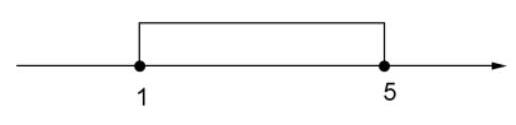
\includegraphics[max width=\textwidth, center]{2024_11_21_9a9f600c3b3af5013d80g-06(2)}\\
C.\\
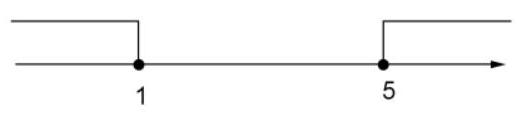
\includegraphics[max width=\textwidth, center]{2024_11_21_9a9f600c3b3af5013d80g-06(5)}\\
B.\\
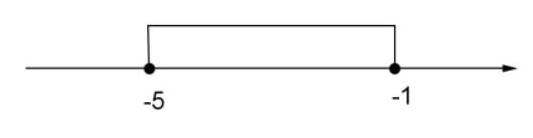
\includegraphics[max width=\textwidth, center]{2024_11_21_9a9f600c3b3af5013d80g-06}\\
D.\\
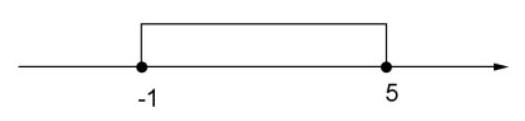
\includegraphics[max width=\textwidth, center]{2024_11_21_9a9f600c3b3af5013d80g-06(6)}

\section*{Zadanie 16. (1 pkt)}
Rozwiązaniami równania \(\frac{\left(x^{2}-4\right)(x-3)}{(x-2)(x+3)}=0\) są liczby:\\
A. \(-3 ;-2 ; 2 ; 3\)\\
B. 2; 3\\
C. \(-3 ; 2\)\\
D. \(-2 ; 3\)

Zadanie 17. (1 pkt)\\
Kąt \(\alpha\) nachylenia ściany bocznej ostrosłupa prawidłowego czworokątnego do płaszczyzny podstawy zaznaczony jest na rysunku:\\
A.\\
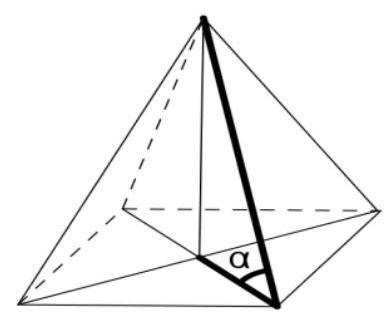
\includegraphics[max width=\textwidth, center]{2024_11_21_9a9f600c3b3af5013d80g-06(7)}\\
C.\\
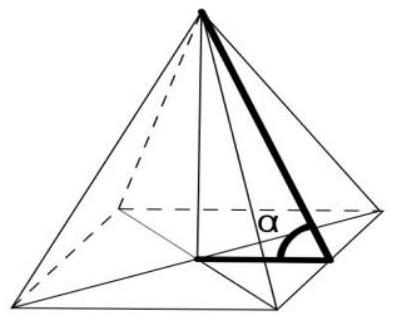
\includegraphics[max width=\textwidth, center]{2024_11_21_9a9f600c3b3af5013d80g-06(4)}\\
B.\\
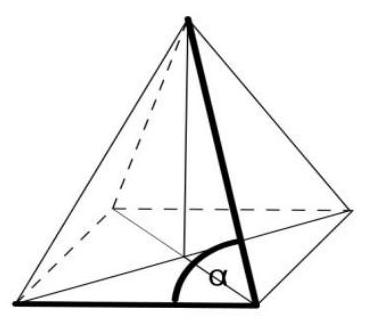
\includegraphics[max width=\textwidth, center]{2024_11_21_9a9f600c3b3af5013d80g-06(1)}\\
D.\\
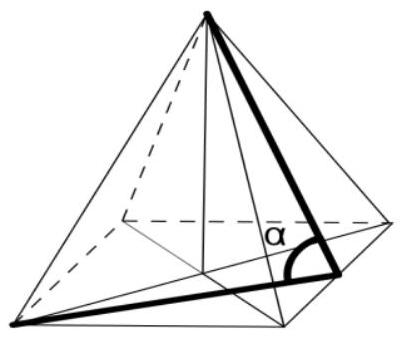
\includegraphics[max width=\textwidth, center]{2024_11_21_9a9f600c3b3af5013d80g-06(3)}

Zadanie 18. (1 pkt)\\
Do wykresu funkcji liniowej \(f\) należą punkty \(A=(4,-3)\) i \(B=(-1,-13)\). Funkcja \(f\) opisana jest wzorem:\\
A. \(f(x)=2 x-11\)\\
B. \(f(x)=2 x+11\)\\
C. \(f(x)=\frac{1}{2} x+1\)\\
D. \(f(x)=\frac{1}{2} x-5\)

Zadanie 19. (1 pkt)\\
Ciągiem arytmetycznym jest ciąg o wyrazie ogólnym \(a_{n}\) równym:\\
A. \(a_{n}=3 \cdot 2^{n}\)\\
B. \(a_{n}=\frac{4 n^{2}-9}{3+2 n}\)\\
C. \(a_{n}=\frac{2 n+3}{n+2}\)\\
D. \(a_{n}=\frac{n^{2}+1}{3}\)

\section*{BRUDNOPIS}
\begin{center}

\includegraphics[max width=\textwidth]{2024_11_21_9a9f600c3b3af5013d80g-07}
\end{center}

Zadanie 20. (1 pkt)\\
Wartość wyrażenia \(\sin ^{2} 23^{\circ}+\sin ^{2} 67^{\circ}\) jest równa:\\
A. \(2 \sin ^{2} 23^{\circ}\)\\
B. \(2 \sin ^{2} 67^{\circ}\)\\
C. 1\\
D. 0

Zadanie 21. (1 pkt)\\
Wszystkich liczb trzycyfrowych parzystych, których cyfra jedności należy do zbioru \(A=\{2,4,5,7\}\), cyfra dziesiątek do zbioru \(B=\{6,7,8\}\), \(a\) cyfra setek do zbioru \(C=\{2,4,5,6\}\) jest:\\
A. 48\\
B. 36\\
C. 24\\
D. 12

Zadanie 22. (1 pkt)\\
Wykres funkcji \(f(x)=2^{x-3}\) przedstawiony jest na rysunku:\\
A.\\
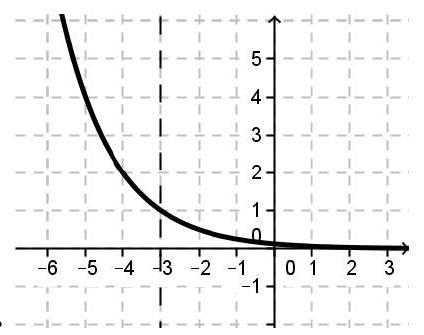
\includegraphics[max width=\textwidth, center]{2024_11_21_9a9f600c3b3af5013d80g-08(3)}\\
C.\\
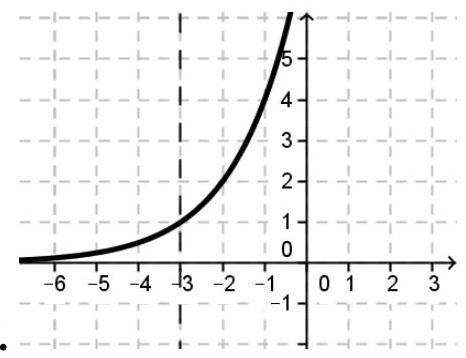
\includegraphics[max width=\textwidth, center]{2024_11_21_9a9f600c3b3af5013d80g-08(2)}\\
B.\\
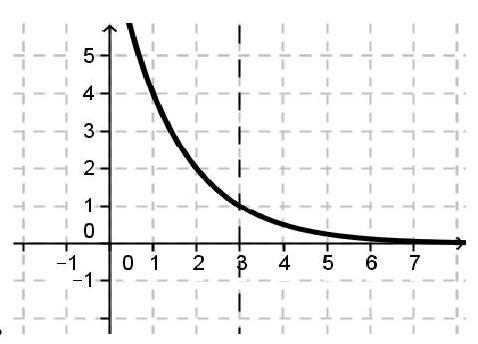
\includegraphics[max width=\textwidth, center]{2024_11_21_9a9f600c3b3af5013d80g-08(1)}\\
D.\\
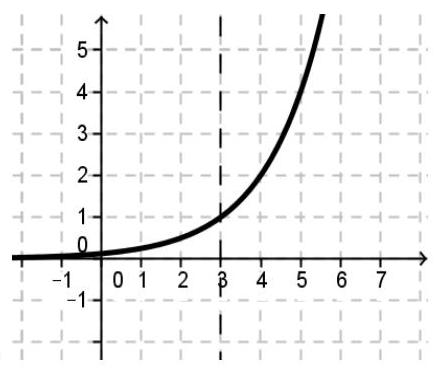
\includegraphics[max width=\textwidth, center]{2024_11_21_9a9f600c3b3af5013d80g-08}

Zadanie 23. (1 pkt)\\
Dany jest okrąg o równaniu \((x+3)^{2}+(y-4)^{2}=25\). Środkiem \(S\) tego okręgu jest punkt:\\
A. \(S=(-3,-4)\)\\
B. \(S=(3,4)\)\\
C. \(S=(3,-4)\)\\
D. \(S=(-3,4)\)

Zadanie 24. (1 pkt)\\
W trapezie miary kątów ostrych są równe \(30^{\circ}\) i \(60^{\circ}\). Wówczas stosunek długości krótszego ramienia do dłuższego jest równy:\\
A. \(\frac{\sqrt{3}}{3}\)\\
B. \(\frac{1}{3}\)\\
C. \(\frac{\sqrt{2}}{2}\)\\
D. \(\frac{1}{2}\)

Zadanie 25. (1 pkt)\\
Największa wartość funkcji \(y=-2 x^{2}+x+1\) w przedziale \(\left\langle-1, \frac{1}{2}\right\rangle\) jest równa:\\
A. \(1 \frac{1}{8}\)\\
B. 1\\
C. \(\frac{1}{4}\)\\
D. -4

\begin{center}
\begin{tabular}{|c|c|c|c|c|c|c|c|c|c|c|c|c|c|c|c|c|c|c|c|c|c|c|c|}
\hline
 &  &  &  &  &  &  &  &  &  &  &  &  &  &  &  &  &  &  &  &  &  &  &  \\
\hline
 &  &  &  &  &  &  &  &  &  &  &  &  &  &  &  &  &  &  &  &  &  &  &  \\
\hline
 &  &  &  &  &  &  &  &  &  &  &  &  &  &  &  &  &  &  &  &  &  &  &  \\
\hline
 &  &  &  &  &  &  &  &  &  &  &  &  &  &  &  &  &  &  &  &  &  &  &  \\
\hline
 &  &  &  &  &  &  &  &  &  &  &  &  &  &  &  &  &  &  &  &  &  &  &  \\
\hline
 &  &  &  &  &  &  &  &  &  &  &  &  &  &  &  &  &  &  &  &  &  &  &  \\
\hline
 &  &  &  &  &  &  &  &  &  &  &  &  &  &  &  &  &  &  &  &  &  &  &  \\
\hline
 &  &  &  &  &  &  &  &  &  &  &  &  &  &  &  &  &  &  &  &  &  &  &  \\
\hline
 &  &  &  &  &  &  &  &  &  &  &  &  &  &  &  &  &  &  &  &  &  &  &  \\
\hline
 &  &  &  &  &  &  &  &  &  &  &  &  &  &  &  &  &  &  &  &  &  &  &  \\
\hline
 &  &  &  &  &  &  &  &  &  &  &  &  &  &  &  &  &  &  &  &  &  &  &  \\
\hline
 &  &  &  &  &  &  &  &  &  &  &  &  &  &  &  &  &  &  &  &  &  &  &  \\
\hline
 &  &  &  &  &  &  &  &  &  &  &  &  &  &  &  &  &  &  &  &  &  &  &  \\
\hline
 &  &  &  &  &  &  &  &  &  &  &  &  &  &  &  &  &  &  &  &  &  &  &  \\
\hline
 &  &  &  &  &  &  &  &  &  &  &  &  &  &  &  &  &  &  &  &  &  &  &  \\
\hline
 &  &  &  &  &  &  &  &  &  &  &  &  &  &  &  &  &  &  &  &  &  &  &  \\
\hline
 &  &  &  &  &  &  &  &  &  &  &  &  &  &  &  &  &  &  &  &  &  &  &  \\
\hline
 &  &  &  &  &  &  &  &  &  &  &  &  &  &  &  &  &  &  &  &  &  &  &  \\
\hline
 &  &  &  &  &  &  &  &  &  &  &  &  &  &  &  &  &  &  &  &  &  &  &  \\
\hline
 &  &  &  &  &  &  &  &  &  &  &  &  &  &  &  &  &  &  &  &  &  &  &  \\
\hline
 &  &  &  &  &  &  &  &  &  &  &  &  &  &  &  &  &  &  &  &  &  &  &  \\
\hline
 &  &  &  &  &  &  &  &  &  &  &  &  &  &  &  &  &  &  &  &  &  &  &  \\
\hline
 &  &  &  &  &  &  &  &  &  &  &  &  &  &  &  &  &  &  &  &  &  &  &  \\
\hline
 &  &  &  &  &  &  &  &  &  &  &  &  &  &  &  &  &  &  &  &  &  &  &  \\
\hline
 &  &  &  &  &  &  &  &  &  &  &  &  &  &  &  &  &  &  &  &  &  &  &  \\
\hline
 &  &  &  &  &  &  &  &  &  &  &  &  &  &  &  &  &  &  &  &  &  &  &  \\
\hline
 &  &  &  &  &  &  &  &  &  &  &  &  &  &  &  &  &  &  &  &  &  &  &  \\
\hline
 &  &  &  &  &  &  &  &  &  &  &  &  &  &  &  &  &  &  &  &  &  &  &  \\
\hline
 &  &  &  &  &  &  &  &  &  &  &  &  &  &  &  &  &  &  &  &  &  &  &  \\
\hline
 &  &  &  &  &  &  &  &  &  &  &  &  &  &  &  &  &  &  &  &  &  &  &  \\
\hline
 &  &  &  &  &  &  &  &  &  &  &  &  &  &  &  &  &  &  &  &  &  &  &  \\
\hline
 &  &  &  &  &  &  &  &  &  &  &  &  &  &  &  &  &  &  &  &  &  &  &  \\
\hline
 &  &  &  &  &  &  &  &  &  &  &  &  &  &  &  &  &  &  &  &  &  &  &  \\
\hline
 &  &  &  &  &  &  &  &  &  &  &  &  &  &  &  &  &  &  &  &  &  &  &  \\
\hline
 &  &  &  &  &  &  &  &  &  &  &  &  &  &  &  &  &  &  &  &  &  &  &  \\
\hline
 &  &  &  &  &  &  &  &  &  &  &  &  &  &  &  &  &  &  &  &  &  &  &  \\
\hline
 &  &  &  &  &  &  &  &  &  &  &  &  &  &  &  &  &  &  &  &  &  &  &  \\
\hline
 &  &  &  &  &  &  &  &  &  &  &  &  &  &  &  &  &  &  &  &  &  &  &  \\
\hline
 &  &  &  &  &  &  &  &  &  &  &  &  &  &  &  &  &  &  &  &  &  &  &  \\
\hline
 &  &  &  &  &  &  &  &  &  &  &  &  &  &  &  &  &  &  &  &  &  &  &  \\
\hline
 &  &  &  &  &  &  &  &  &  &  &  &  &  &  &  &  &  &  &  &  &  &  &  \\
\hline
 &  &  &  &  &  &  &  &  &  &  &  &  &  &  &  &  &  &  &  &  &  &  &  \\
\hline
 &  &  &  &  &  &  &  &  &  &  &  &  &  &  &  &  &  &  &  &  &  &  &  \\
\hline
 &  &  &  &  &  &  &  &  &  &  &  &  &  &  &  &  &  &  &  &  &  &  &  \\
\hline
 &  &  &  &  &  &  &  &  &  &  &  &  &  &  &  &  &  &  &  &  &  &  &  \\
\hline
\end{tabular}
\end{center}

\section*{ZADANIA OTWARTE}
\section*{Rozwiąania zadań o numerach od 26. do 34. należ̀ zapisać w wyznaczonych miejscach pod treścią zadania.}
Zadanie 26. (2 pkt)\\
Rozwiąż nierówność: \(-x^{2}+2 x+8 \geq 0\).

\begin{center}
\begin{tabular}{|c|c|c|c|c|c|c|c|c|c|c|c|c|c|c|c|c|c|c|c|c|c|c|c|c|c|c|c|c|c|}
\hline
 &  &  &  &  &  &  &  &  &  &  &  &  &  &  &  &  &  &  &  &  &  &  &  &  &  &  &  &  &  \\
\hline
 &  &  &  &  &  &  &  &  &  &  &  &  &  &  &  &  &  &  &  &  &  &  &  &  &  &  &  &  &  \\
\hline
 &  &  &  &  &  &  &  &  &  &  &  &  &  &  &  &  &  &  &  &  &  &  &  &  &  &  &  &  &  \\
\hline
 &  &  &  &  &  &  &  &  &  &  &  &  &  &  &  &  &  &  &  &  &  &  &  &  &  &  &  &  &  \\
\hline
 &  &  &  &  &  &  &  &  &  &  &  &  &  &  &  &  &  &  &  &  &  &  &  &  &  &  &  &  &  \\
\hline
 &  &  &  &  &  &  &  &  &  &  &  &  &  &  &  &  &  &  &  &  &  &  &  &  &  &  &  &  &  \\
\hline
 &  &  &  &  &  &  &  &  &  &  &  &  &  &  &  &  &  &  &  &  &  &  &  &  &  &  &  &  &  \\
\hline
 &  &  &  &  &  &  &  &  &  &  &  &  &  &  &  &  &  &  &  &  &  &  &  &  &  &  &  &  &  \\
\hline
 &  &  &  &  &  &  &  &  &  &  &  &  &  &  &  &  &  &  &  &  &  &  &  &  &  &  &  &  &  \\
\hline
 &  &  &  &  &  &  &  &  &  &  &  &  &  &  &  &  &  &  &  &  &  &  &  &  &  &  &  &  &  \\
\hline
 &  &  &  &  &  &  &  &  &  &  &  &  &  &  &  &  &  &  &  &  &  &  &  &  &  &  &  &  &  \\
\hline
 &  &  &  &  &  &  &  &  &  &  &  &  &  &  &  &  &  &  &  &  &  &  &  &  &  &  &  &  &  \\
\hline
 &  &  &  &  &  &  &  &  &  &  &  &  &  &  &  &  &  &  &  &  &  &  &  &  &  &  &  &  &  \\
\hline
 &  &  &  &  &  &  &  &  &  &  &  &  &  &  &  &  &  &  &  &  &  &  &  &  &  &  &  &  &  \\
\hline
 &  &  &  &  &  &  &  &  &  &  &  &  &  &  &  &  &  &  &  &  &  &  &  &  & 
\includegraphics[max width=\textwidth]{2024_11_21_9a9f600c3b3af5013d80g-10}
 &  &  &  & - \\
\hline
\end{tabular}
\end{center}

Odpowiedź:\\
Zadanie 27. (2 pkt)\\
Na boku \(D C\) kwadratu \(A B C D\) obrano punkt \(K\) tak, że \(|D K|=|K C|\) (rys.). Przekątna \(A C\) kwadratu przecina odcinek \(B K\) w punkcie \(P\). Uzasadnij, że pole trójkąta \(A B P\) jest czterokrotnie większe niż pole trójkąta \(K C P\).\\
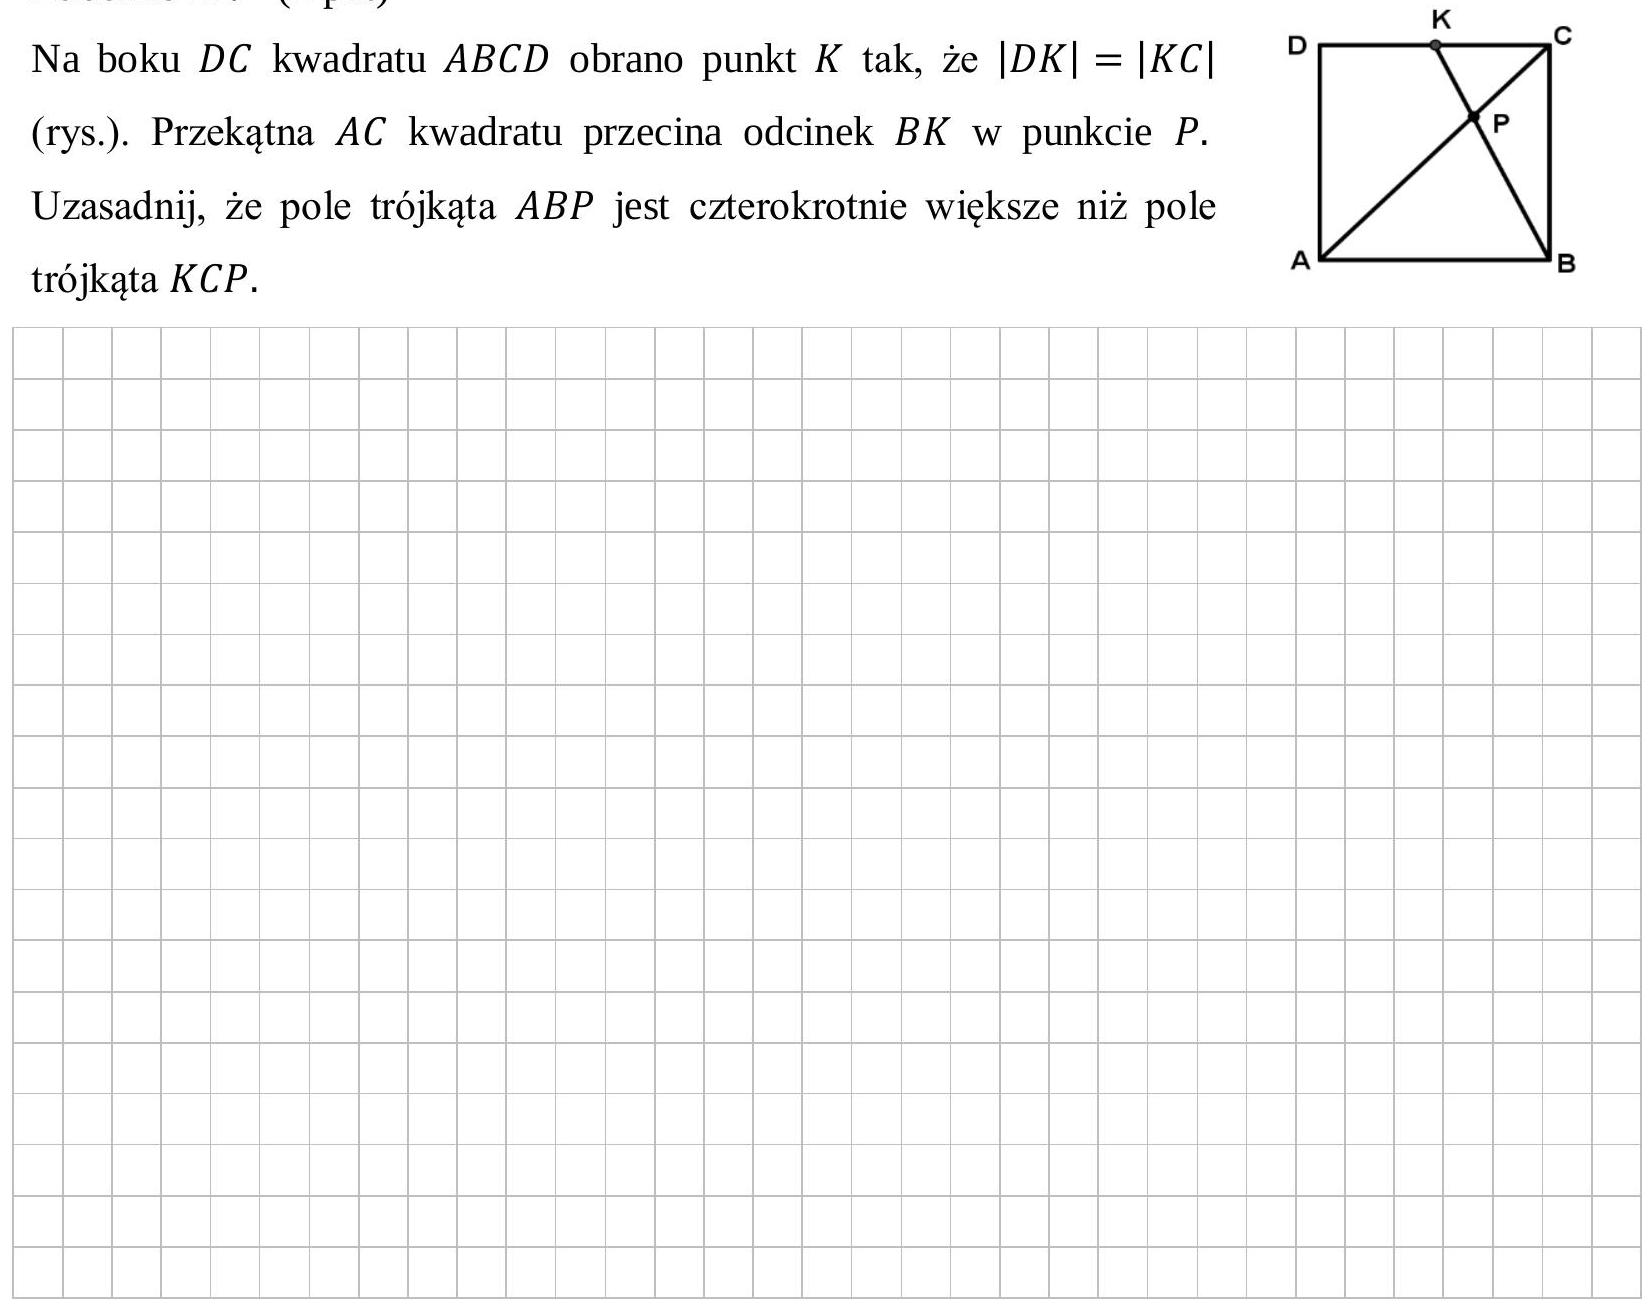
\includegraphics[max width=\textwidth, center]{2024_11_21_9a9f600c3b3af5013d80g-10(1)}

Zadanie 28. (2 pkt)\\
Oblicz pierwszy wyraz i iloraz ciągu geometrycznego wiedząc, że trzeci wyraz jest równy 18, a szósty 486.

\begin{center}
\begin{tabular}{|c|c|c|c|c|c|c|c|c|c|c|c|c|c|c|c|c|c|c|c|c|c|c|c|c|c|}
\hline
 &  &  &  &  &  &  &  &  &  &  &  &  &  &  &  &  &  &  &  &  &  &  &  &  &  \\
\hline
 &  &  &  &  &  &  &  &  &  &  &  &  &  &  &  &  &  &  &  &  &  &  &  &  &  \\
\hline
 &  &  &  &  &  &  &  &  &  &  &  &  &  &  &  &  &  &  &  &  &  &  &  &  &  \\
\hline
 &  &  &  &  &  &  &  &  &  &  &  &  &  &  &  &  &  &  &  &  &  &  &  &  &  \\
\hline
 &  &  &  &  &  &  &  &  &  &  &  &  &  &  &  &  &  &  &  &  &  &  &  &  &  \\
\hline
 &  &  &  &  &  &  &  &  &  &  &  &  &  &  &  &  &  &  &  &  &  &  &  &  &  \\
\hline
 &  &  &  &  &  &  &  &  &  &  &  &  &  &  &  &  &  &  &  &  &  &  &  &  &  \\
\hline
 &  &  &  &  &  &  &  &  &  &  &  &  &  &  &  &  &  &  &  &  &  &  &  &  &  \\
\hline
 &  &  &  &  &  &  &  &  &  &  &  &  &  &  &  &  &  &  &  &  &  &  &  &  &  \\
\hline
 &  &  &  &  &  &  &  &  &  &  &  &  &  &  &  &  &  &  &  &  &  &  &  &  &  \\
\hline
 &  &  &  &  &  &  &  &  &  &  &  &  &  &  &  &  &  &  &  &  &  &  &  &  &  \\
\hline
 &  &  &  &  &  &  &  &  &  &  &  &  &  &  &  &  &  &  &  &  &  &  &  &  &  \\
\hline
 &  &  &  &  &  &  &  &  &  &  &  &  &  &  &  &  &  &  &  &  &  &  &  &  &  \\
\hline
 &  &  &  &  &  &  &  &  &  &  &  &  &  &  &  &  &  &  &  &  &  &  &  &  &  \\
\hline
 &  &  &  &  &  &  &  &  &  &  &  &  &  &  &  &  &  &  &  &  &  &  &  &  &  \\
\hline
 &  &  &  &  &  &  &  &  &  &  &  &  &  &  &  &  &  &  &  &  &  &  &  &  &  \\
\hline
 &  &  &  &  &  &  &  &  &  &  &  &  &  &  &  &  &  &  &  &  &  &  &  &  &  \\
\hline
 &  &  &  &  &  &  &  &  &  &  &  &  &  &  &  &  &  &  &  &  &  &  &  &  &  \\
\hline
\end{tabular}
\end{center}

\section*{Odpowiedź:}
Zadanie 29. (2 pkt)\\
Wykaż, że liczby \(a=\frac{-5}{2 \sqrt{2}+3}\) oraz \(b=|10 \sqrt{2}-15|\) są liczbami przeciwnymi.\\

\includegraphics[max width=\textwidth, center]{2024_11_21_9a9f600c3b3af5013d80g-11}

\section*{Zadanie 30. (2 pkt)}
W trójkącie równoramiennym \(A B C\) o podstawie \(A B\) poprowadzono wysokość z wierzchołka C. Wyznacz równanie prostej zawierającej tę wysokość, jeśli \(A=(2,8), B=(-2,4)\).\\

\includegraphics[max width=\textwidth, center]{2024_11_21_9a9f600c3b3af5013d80g-12(1)}

Odpowiedź:\\
Zadanie 31. (2 pkt)\\
Ze zbioru liczb \(\{1,2,3,4,5\}\) losujemy kolejno trzy razy po jednej liczbie bez zwracania tworząc liczbę trzycyfrową. Oblicz prawdopodobieństwo zdarzenia A - otrzymana liczba jest mniejsza od 432.\\

\includegraphics[max width=\textwidth, center]{2024_11_21_9a9f600c3b3af5013d80g-12}

Zadanie 32. (4 pkt)\\
Z miast A i B odległych o 330 km wyjechały naprzeciwko siebie dwa samochody. Samochód jadący z miasta A wyjechał 20 minut wcześniej i jechał z prędkością o \(9 \mathrm{~km} / \mathrm{h}\) mniejszą niż samochód jadący z miasta B. Samochody te minęły się w odległości 168 km licząc od miasta A. Oblicz średnią prędkość każdego z samochodów.\\

\includegraphics[max width=\textwidth, center]{2024_11_21_9a9f600c3b3af5013d80g-13}

Zadanie 33. (4 pkt)\\
Oblicz pole i obwód rombu \(A B C D\) wiedząc, że przekątna \(A C\) jest zawarta w prostej o równaniu \(y=2 x-2\) oraz \(A=(-1,-4)\) i \(D=(-6,6)\).\\

\includegraphics[max width=\textwidth, center]{2024_11_21_9a9f600c3b3af5013d80g-14}

Odpowiedź:

Zadanie 34. (5 pkt)\\
Metalowy stożek, którego tworząca o długości 10 jest nachylona do płaszczyzny podstawy pod kątem \(30^{\circ}\), przetopiono na sześć jednakowych kulek. Oblicz promień kulki.\\

\includegraphics[max width=\textwidth, center]{2024_11_21_9a9f600c3b3af5013d80g-15}

Odpowiedź:

\section*{PESEL}
WYPEとNIA ZDAJĄCY

\begin{center}
\begin{tabular}{|c|c|c|c|c|}
\hline
\multirow{2}{*}{\begin{tabular}{l}
Nr \\
zad. \\
\end{tabular}} & \multicolumn{4}{|c|}{Odpowiedzi} \\
\hline
 & A & B & C & D \\
\hline
1 & \(\square\) & ■ & ■ & ■ \\
\hline
2 & ㅁ & ㅁ & ㅁ & \(\square\) \\
\hline
3 & \(\square\) & ㅁ & ㅁ & \(\square\) \\
\hline
4 & ㅁ & ㅁ & ㅁ & ㅁ \\
\hline
5 & \(\square\) & ㅁ & ■ & - \\
\hline
6 & \(\square\) & ㅁ & ㅁ & \(\square\) \\
\hline
7 & - & ㅁ & ㅁ & ㅁ \\
\hline
8 & - & ■ & - & - \\
\hline
9 & ㅁ & ㅁ & ㅁ & ㅁ \\
\hline
10 & ㅁ & ㅁ & \(\square\) & \(\square\) \\
\hline
11 & ■ & ㅁ & ㅁ & ㅁ \\
\hline
12 & \(\square\) & \(\square\) & \(\square\) & ■ \\
\hline
13 & \(\square\) & ㅁ & ㅁ & \(\square\) \\
\hline
14 & \(\square\) & ㅁ & ■ & \(\square\) \\
\hline
15 & ㅁ & ㅁ & ■ & ㅁ \\
\hline
16 & ㅁ & ㅁ & ㅁ & ㅁ \\
\hline
17 & ㅁ & ㅁ & \(\square\) & \(\square\) \\
\hline
18 & \(\square\) & ㅁ & \(\square\) & - \\
\hline
19 & \(\square\) & ㅁ & ■ & \(\square\) \\
\hline
20 & ㅁ & ㅁ & ㅁ & ㅁ \\
\hline
21 & ㅁ & ㅁ & ㅁ & ㅁ \\
\hline
22 & \(\square\) & ㅁ & ■ & ■ \\
\hline
23 & \(\square\) & ㅁ & ㅁ & \(\square\) \\
\hline
24 & ㅁ & ㅁ & ㅁ & ㅁ \\
\hline
25 & \(\square\) & ㅁ & ■ & ■ \\
\hline
\end{tabular}
\end{center}

WYPEŁNIA EGZAMINATOR

\begin{center}
\begin{tabular}{|c|c|c|c|c|c|c|}
\hline
\multirow{2}{*}{\begin{tabular}{c}
Nr \\
zad. \\
\end{tabular}} & \multicolumn{6}{|c|}{Punkty} \\
\hline
 & \(\mathbf{0}\) & \(\mathbf{1}\) & \(\mathbf{2}\) & \(\mathbf{3}\) & \(\mathbf{4}\) & \(\mathbf{5}\) \\
\hline
\(\mathbf{2 6}\) & \(\square\) & \(\square\) & \(\square\) &  &  &  \\
\hline
\(\mathbf{2 7}\) & \(\square\) & \(\square\) & \(\square\) &  &  &  \\
\hline
\(\mathbf{2 8}\) & \(\square\) & \(\square\) & \(\square\) &  &  &  \\
\hline
\(\mathbf{2 9}\) & \(\square\) & \(\square\) & \(\square\) &  &  &  \\
\hline
\(\mathbf{3 0}\) & \(\square\) & \(\square\) & \(\square\) &  &  &  \\
\hline
\(\mathbf{3 1}\) & \(\square\) & \(\square\) & \(\square\) &  &  &  \\
\hline
\(\mathbf{3 2}\) & \(\square\) & \(\square\) & \(\square\) & \(\square\) & \(\square\) &  \\
\hline
\(\mathbf{3 3}\) & \(\square\) & \(\square\) & \(\square\) & \(\square\) & \(\square\) &  \\
\hline
\(\mathbf{3 4}\) & \(\square\) & \(\square\) & \(\square\) & \(\square\) & \(\square\) & \(\square\) \\
\hline
\end{tabular}
\end{center}

SUMA PUNKTÓW\\

\includegraphics[max width=\textwidth, center]{2024_11_21_9a9f600c3b3af5013d80g-16}


\end{document}